\let\negmedspace\undefined
\let\negthickspace\undefined
\documentclass[journal]{IEEEtran}
\usepackage[a5paper, margin=10mm, onecolumn]{geometry}
%\usepackage{lmodern} % Ensure lmodern is loaded for pdflatex
\usepackage{tfrupee} % Include tfrupee package

\setlength{\headheight}{1cm} % Set the height of the header box
\setlength{\headsep}{0mm}     % Set the distance between the header box and the top of the text

\usepackage{gvv-book}
\usepackage{gvv}
\usepackage{cite}
\usepackage{amsmath,amssymb,amsfonts,amsthm}
\usepackage{algorithmic}
\usepackage{graphicx}
\usepackage{textcomp}
\usepackage{xcolor}
\usepackage{txfonts}
\usepackage{listings}
\usepackage{enumitem}
\usepackage{mathtools}
\usepackage{gensymb}
\usepackage{comment}
\usepackage[breaklinks=true]{hyperref}
\usepackage{tkz-euclide} 
\usepackage{listings}
% \usepackage{gvv}                                        
\def\inputGnumericTable{}                                 
\usepackage[latin1]{inputenc}                                
\usepackage{color}                                            
\usepackage{array}                                            
\usepackage{longtable}                                       
\usepackage{calc}                                             
\usepackage{multirow}                                         
\usepackage{hhline}                                           
\usepackage{ifthen}                                           
\usepackage{lscape}
\usepackage{circuitikz}
\tikzstyle{block} = [rectangle, draw, fill=blue!20, 
    text width=4em, text centered, rounded corners, minimum height=3em]
\tikzstyle{sum} = [draw, fill=blue!10, circle, minimum size=1cm, node distance=1.5cm]
\tikzstyle{input} = [coordinate]
\tikzstyle{output} = [coordinate]



\graphicspath{{figs/}}
\renewcommand{\theequation}{2.4.19.\arabic{equation}}
\renewcommand{\thefigure}{2.4.19.\arabic{figure}}

\bibliographystyle{IEEEtran}
\vspace{1.5em}

\title{2.4.19}
\author{E Achyuta Siddartha - ee25btech11024}

\begin{document}
\maketitle

\noindent
\textbf{Problem Statement} \\
If $\vec{A}, \vec{B}, \vec{C}, \vec{D}$ are the points with position vectors $\hat{i}+\hat{j}-\hat{k}$, $2\hat{i}-\hat{j}+3\hat{k}$, $2\hat{i}-3\hat{k}$, $3\hat{i}-2\hat{j}+\hat{k}$ respectively, find the projection of AB along CD.

\vspace{1.5em}

\noindent
\textbf{Solution:}\\

\begin{center}
    \begin{tabular}{|c|c|c|}
    \hline
    \textbf{Symbol} & \textbf{Value} & \textbf{Description}  \\
    \hline
    \textbf{\vec{A}}      & \myvec{1 \\ 1\\-1}         & First Point\\
    \hline
    \textbf{\vec{B}}      & \myvec{2 \\ -1 \\3}        & Second Point\\
    \hline
    \textbf{\vec{C}}      & \myvec{2 \\ 0 \\-3}        &Third Point \\
    \hline
    \textbf{\vec{D}}      & \myvec{3 \\ -2 \\1}        &Fourth Point \\
    \hline
    \end{tabular}
\end{center}
\noindent

\noindent
From the the given points we find AB and CD
\begin{align}
\vec{B} - \vec{A} = \myvec{1 \\ 2 \\-4}, \vec{D} - \vec{C} = \myvec{1 \\ 2 \\-4}
\label{eq:2.4.19.1}
\end{align}


Let P be the projection of AB along CD. We know that
\begin{align}
    \vec{P} = (\frac{(\vec{B} - \vec{A})^\top (\vec{D} - \vec{C})}{\|\vec{D} - \vec{C}\|^2}) (\vec{D} - \vec{C})
    \label{eq:2.4.19.2}
\end{align}

Substituting \eqref{eq:2.4.19.1} in \eqref{eq:2.4.19.2} we get
\begin{align}
    P = (\vec{D} - \vec{C}) =  \myvec{1 \\ 2 \\-4}
\end{align}

 Thus, the projection of AB along CD = $\myvec{1 \\ 2 \\-4}\\$

See Figure~\ref{fig:3DVectors}.

\begin{figure}[h!]
    \centering
    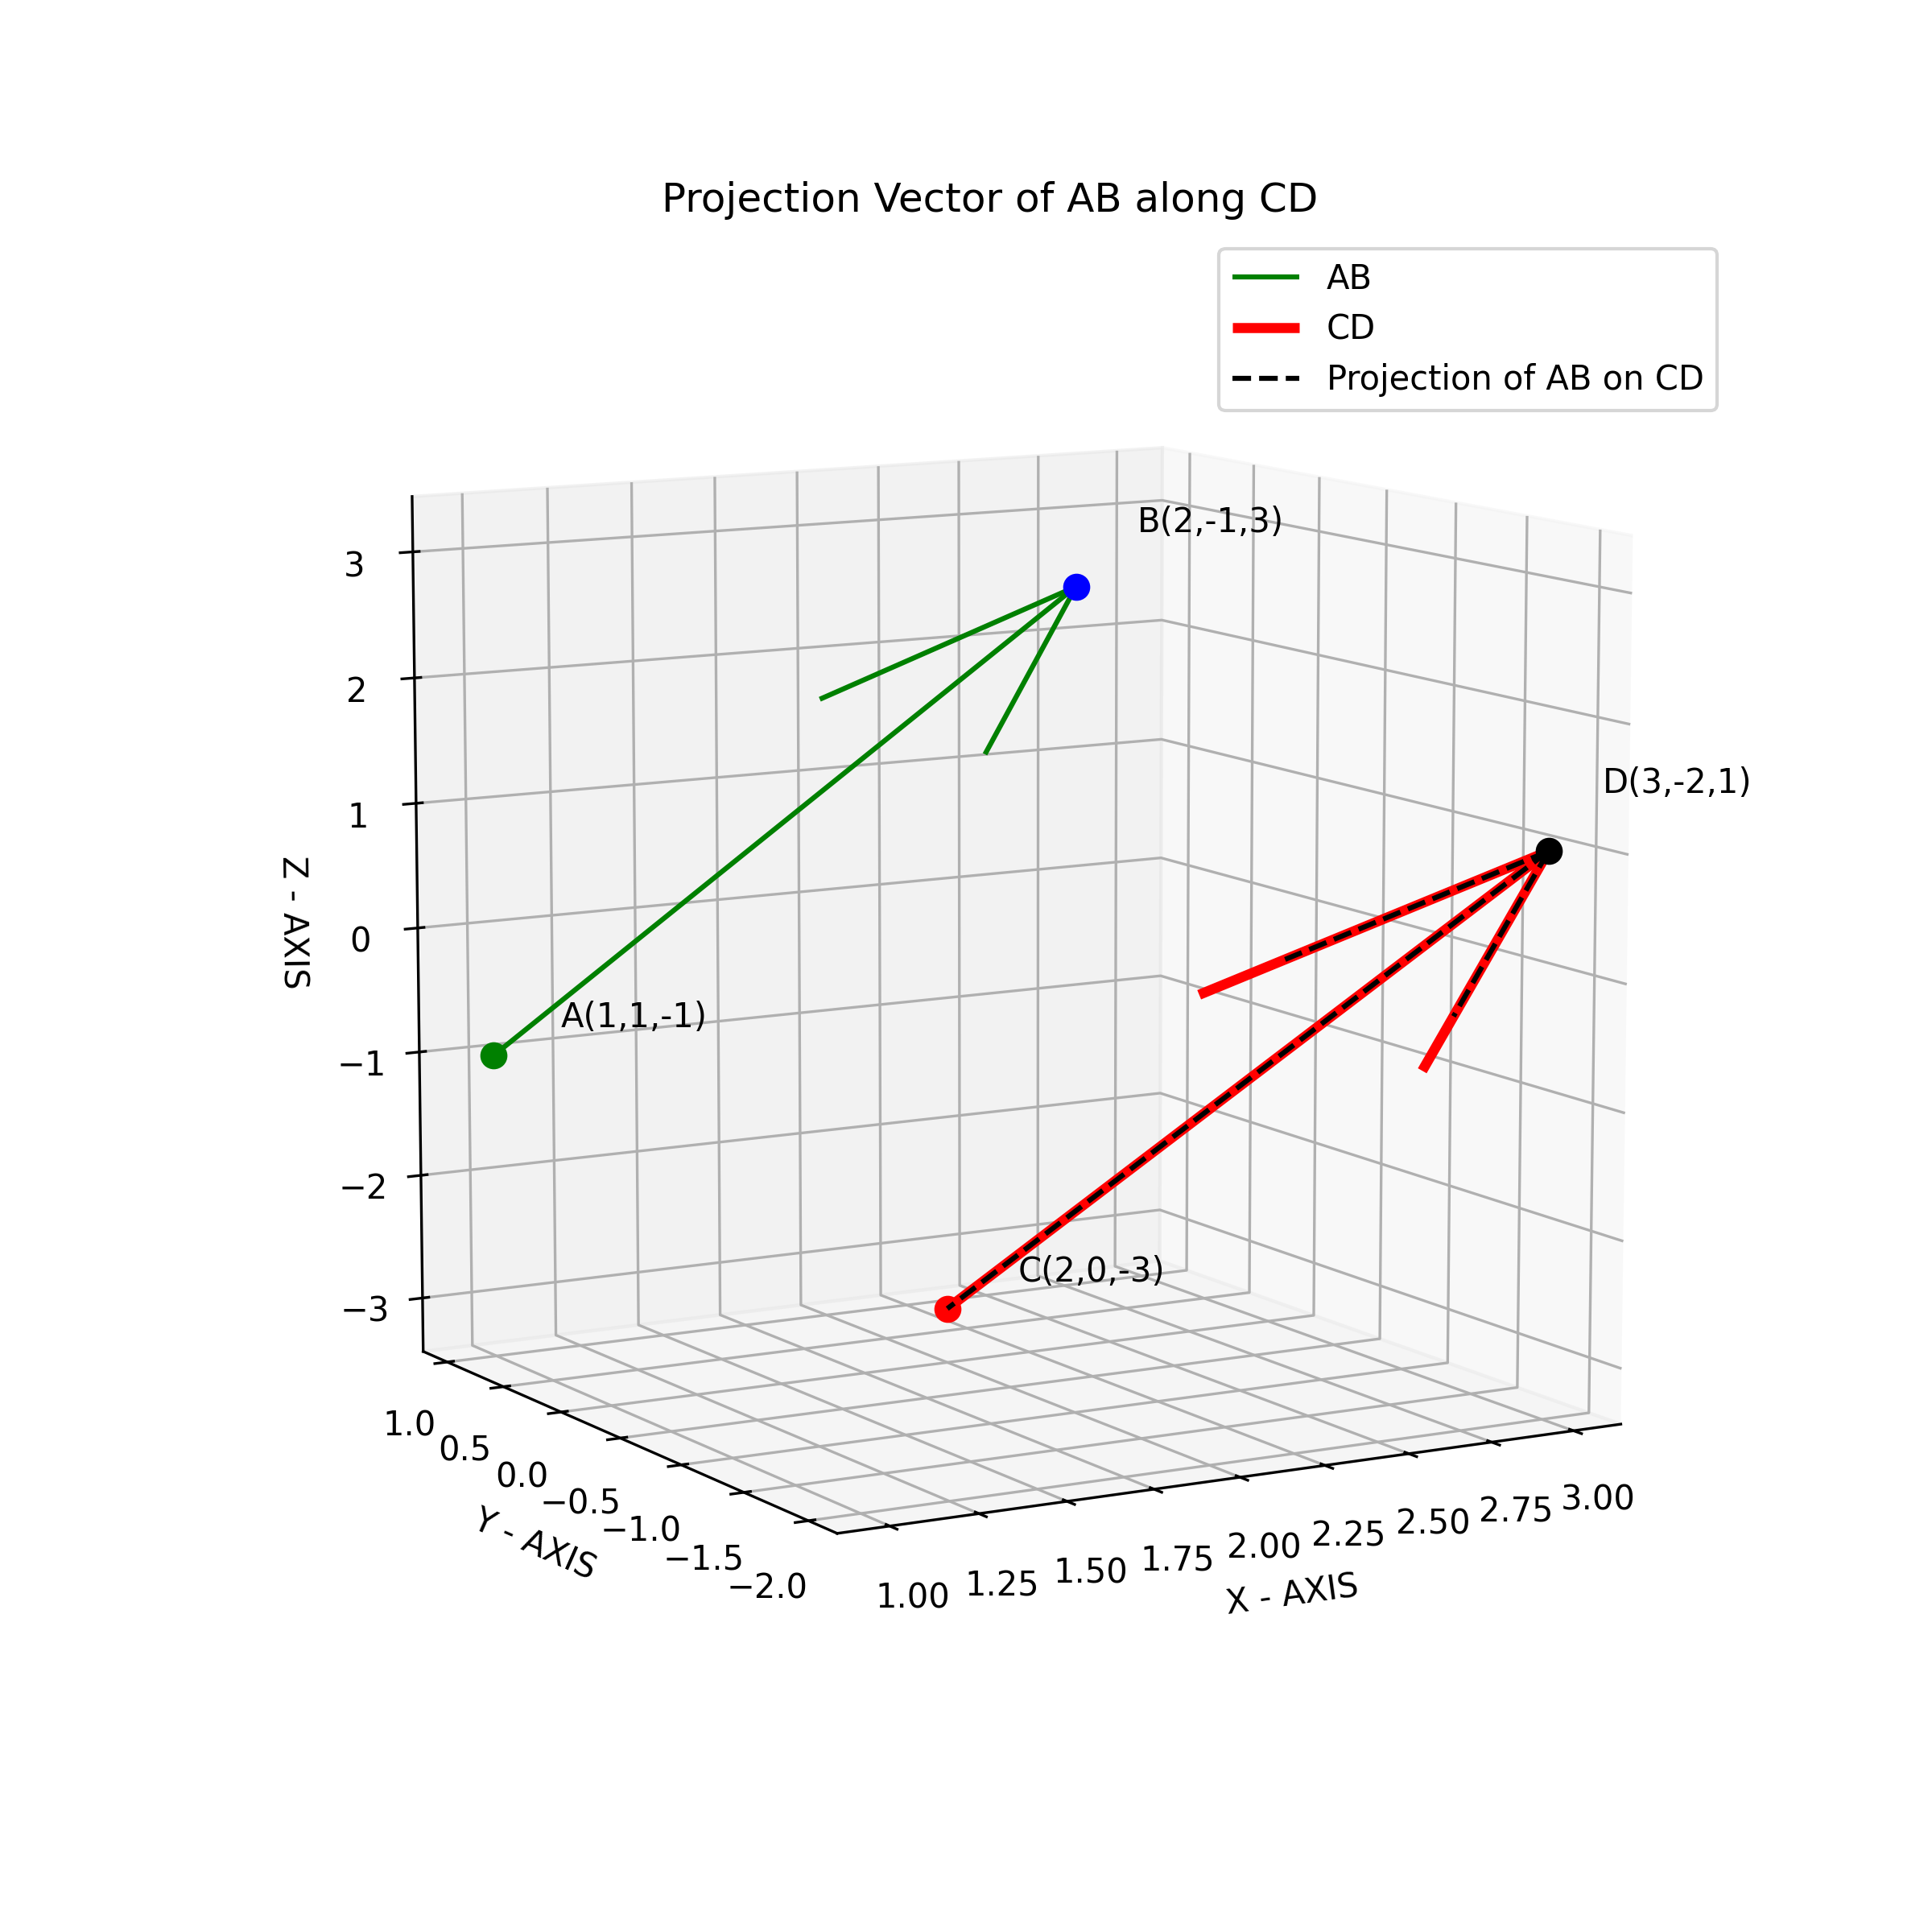
\includegraphics[width=1.0\linewidth]{figs/fig.png}
    \caption{}
    \label{fig:3DVectors}
\end{figure}

\end{document}
